\documentclass{whiteboard}
\begin{document}
\begin{frame}[plain,t]
\bbcover{Programação Lógica}{Recursão}{Prof. Edson Alves}{Campus UnB Gama: Faculdade de Ciências e Tecnologias em Engenharia}

\end{frame}
\begin{frame}[plain,t]
\begin{tikzpicture}
\node[draw,opacity=0] at (0, 0) {x};
\node[draw,opacity=0] at (14, 8) {x};

	\node[anchor=west] (title) at (0.0, 7.0) { \Large \bbbold{Recursão em Prolog} };

\end{tikzpicture}
\end{frame}
\begin{frame}[plain,t]
\begin{tikzpicture}
\node[draw,opacity=0] at (0, 0) {x};
\node[draw,opacity=0] at (14, 8) {x};

	\node[anchor=west] (title) at (0.0, 7.0) { \Large \bbbold{Recursão em Prolog} };

	\node[anchor=west] (a) at (1.0, 6.0) { $\star$ \bbtext{Em Prolog, predicados podem ser definidos recursivamente} };

\end{tikzpicture}
\end{frame}
\begin{frame}[plain,t]
\begin{tikzpicture}
\node[draw,opacity=0] at (0, 0) {x};
\node[draw,opacity=0] at (14, 8) {x};

	\node[anchor=west] (title) at (0.0, 7.0) { \Large \bbbold{Recursão em Prolog} };

	\node[anchor=west] (a) at (1.0, 6.0) { $\star$ \bbtext{Em Prolog, predicados podem ser definidos recursivamente} };

	\node[anchor=west] (b) at (1.0, 5.0) { $\star$ \bbtext{Um predicado é definido \bbbold{recursivamente} se uma ou mais regras em sua definição} };

	\node[anchor=west] (b1) at (0.5, 4.5) { \bbtext{se referem ao próprio predicado} };

\end{tikzpicture}
\end{frame}
\begin{frame}[plain,t]
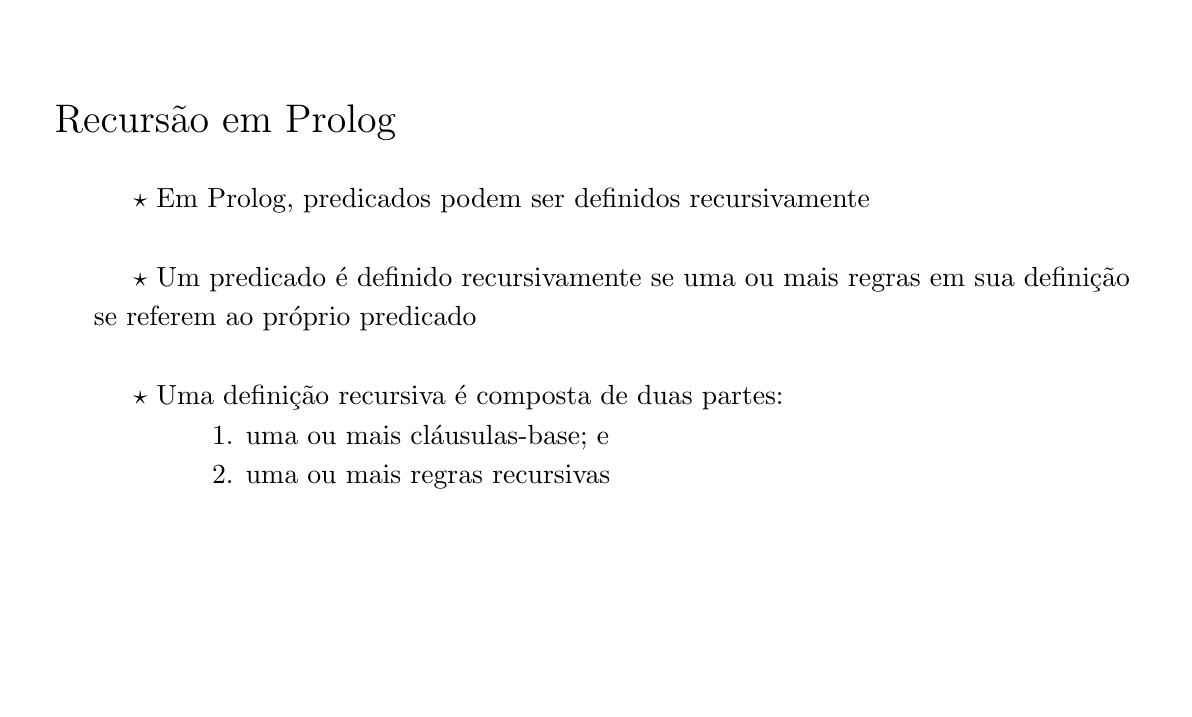
\begin{tikzpicture}
\node[draw,opacity=0] at (0, 0) {x};
\node[draw,opacity=0] at (14, 8) {x};

	\node[anchor=west] (title) at (0.0, 7.0) { \Large \bbbold{Recursão em Prolog} };

	\node[anchor=west] (a) at (1.0, 6.0) { $\star$ \bbtext{Em Prolog, predicados podem ser definidos recursivamente} };

	\node[anchor=west] (b) at (1.0, 5.0) { $\star$ \bbtext{Um predicado é definido \bbbold{recursivamente} se uma ou mais regras em sua definição} };

	\node[anchor=west] (b1) at (0.5, 4.5) { \bbtext{se referem ao próprio predicado} };

	\node[anchor=west] (c) at (1.0, 3.5) { $\star$ \bbtext{Uma definição recursiva é composta de duas partes:} };

	\node[anchor=west] (c1) at (2.0, 3.0) { \bbbold{1.} \bbtext{uma ou mais cláusulas-base; e} };

	\node[anchor=west] (c2) at (2.0, 2.5) { \bbbold{2.} \bbtext{uma ou mais regras recursivas} };

\end{tikzpicture}
\end{frame}
\begin{frame}[plain,t]
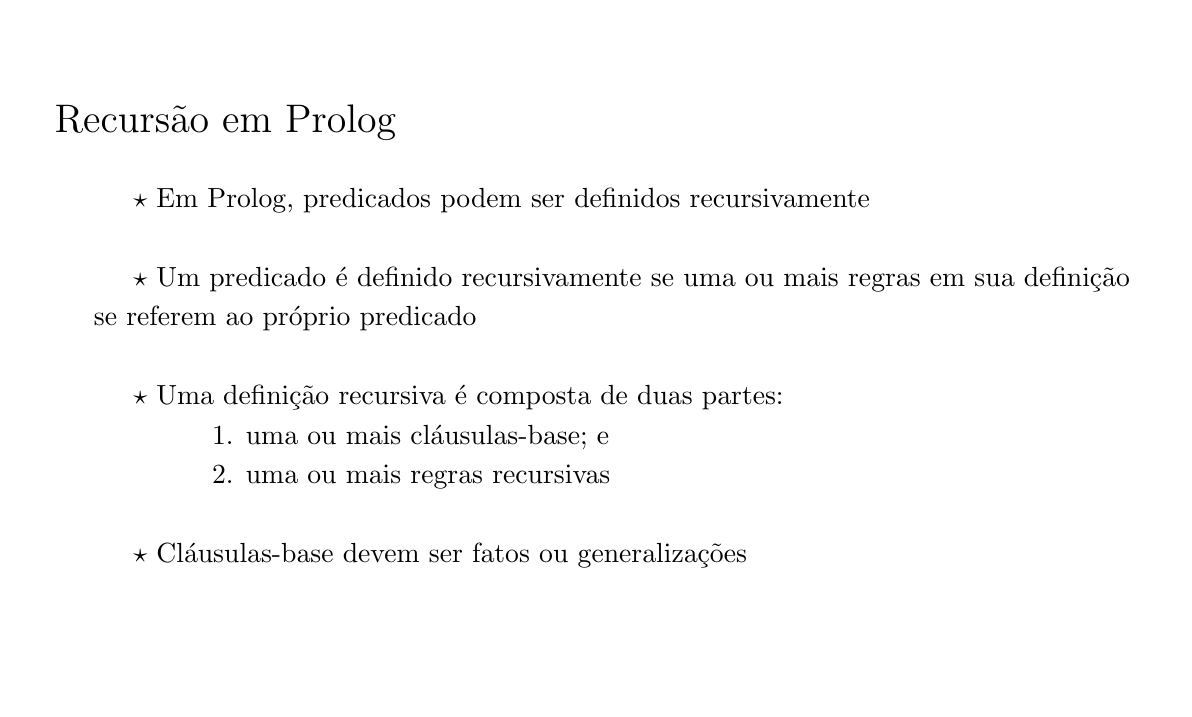
\begin{tikzpicture}
\node[draw,opacity=0] at (0, 0) {x};
\node[draw,opacity=0] at (14, 8) {x};

	\node[anchor=west] (title) at (0.0, 7.0) { \Large \bbbold{Recursão em Prolog} };

	\node[anchor=west] (a) at (1.0, 6.0) { $\star$ \bbtext{Em Prolog, predicados podem ser definidos recursivamente} };

	\node[anchor=west] (b) at (1.0, 5.0) { $\star$ \bbtext{Um predicado é definido \bbbold{recursivamente} se uma ou mais regras em sua definição} };

	\node[anchor=west] (b1) at (0.5, 4.5) { \bbtext{se referem ao próprio predicado} };

	\node[anchor=west] (c) at (1.0, 3.5) { $\star$ \bbtext{Uma definição recursiva é composta de duas partes:} };

	\node[anchor=west] (c1) at (2.0, 3.0) { \bbbold{1.} \bbtext{uma ou mais cláusulas-base; e} };

	\node[anchor=west] (c2) at (2.0, 2.5) { \bbbold{2.} \bbtext{uma ou mais regras recursivas} };

	\node[anchor=west] (d) at (1.0, 1.5) { $\star$ \bbtext{Cláusulas-base devem ser fatos ou generalizações} };

\end{tikzpicture}
\end{frame}
\begin{frame}[plain,t]
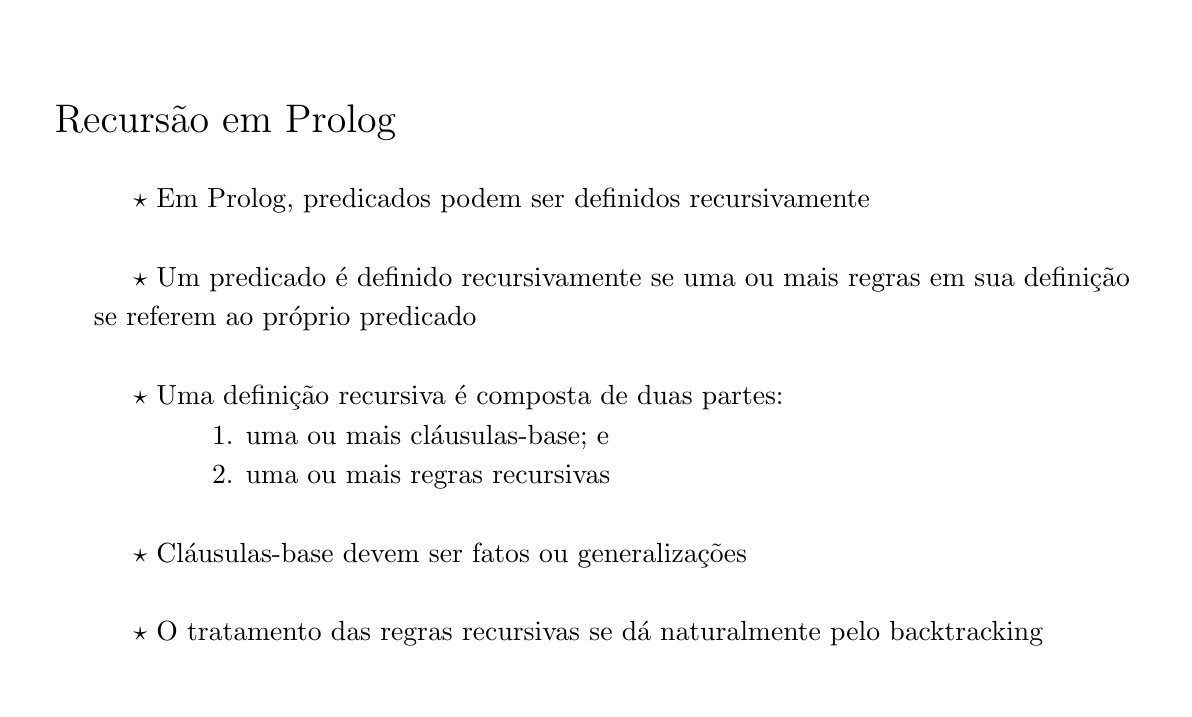
\begin{tikzpicture}
\node[draw,opacity=0] at (0, 0) {x};
\node[draw,opacity=0] at (14, 8) {x};

	\node[anchor=west] (title) at (0.0, 7.0) { \Large \bbbold{Recursão em Prolog} };

	\node[anchor=west] (a) at (1.0, 6.0) { $\star$ \bbtext{Em Prolog, predicados podem ser definidos recursivamente} };

	\node[anchor=west] (b) at (1.0, 5.0) { $\star$ \bbtext{Um predicado é definido \bbbold{recursivamente} se uma ou mais regras em sua definição} };

	\node[anchor=west] (b1) at (0.5, 4.5) { \bbtext{se referem ao próprio predicado} };

	\node[anchor=west] (c) at (1.0, 3.5) { $\star$ \bbtext{Uma definição recursiva é composta de duas partes:} };

	\node[anchor=west] (c1) at (2.0, 3.0) { \bbbold{1.} \bbtext{uma ou mais cláusulas-base; e} };

	\node[anchor=west] (c2) at (2.0, 2.5) { \bbbold{2.} \bbtext{uma ou mais regras recursivas} };

	\node[anchor=west] (d) at (1.0, 1.5) { $\star$ \bbtext{Cláusulas-base devem ser fatos ou generalizações} };

	\node[anchor=west] (e) at (1.0, 0.5) { $\star$ \bbtext{O tratamento das regras recursivas se dá naturalmente pelo \bbenglish{backtracking}} };

\end{tikzpicture}
\end{frame}
\begin{frame}[plain,t]
\vspace*{\fill}

\inputcode{prolog}{codes/fact.pl}

\vspace*{\fill}
\end{frame}
\begin{frame}[plain,t]
\begin{tikzpicture}
\node[draw,opacity=0] at (0, 0) {x};
\node[draw,opacity=0] at (14, 8) {x};

	\node[anchor=west] (title) at (0.0, 7.0) { \Large \bbbold{Características da recursão em Prolog} };

\end{tikzpicture}
\end{frame}
\begin{frame}[plain,t]
\begin{tikzpicture}
\node[draw,opacity=0] at (0, 0) {x};
\node[draw,opacity=0] at (14, 8) {x};

	\node[anchor=west] (title) at (0.0, 7.0) { \Large \bbbold{Características da recursão em Prolog} };

	\node[anchor=west] (a) at (1.0, 6.0) { $\star$ \bbtext{Cada nível de recursão tem seu próprio conjunto de variáveis} };

\end{tikzpicture}
\end{frame}
\begin{frame}[plain,t]
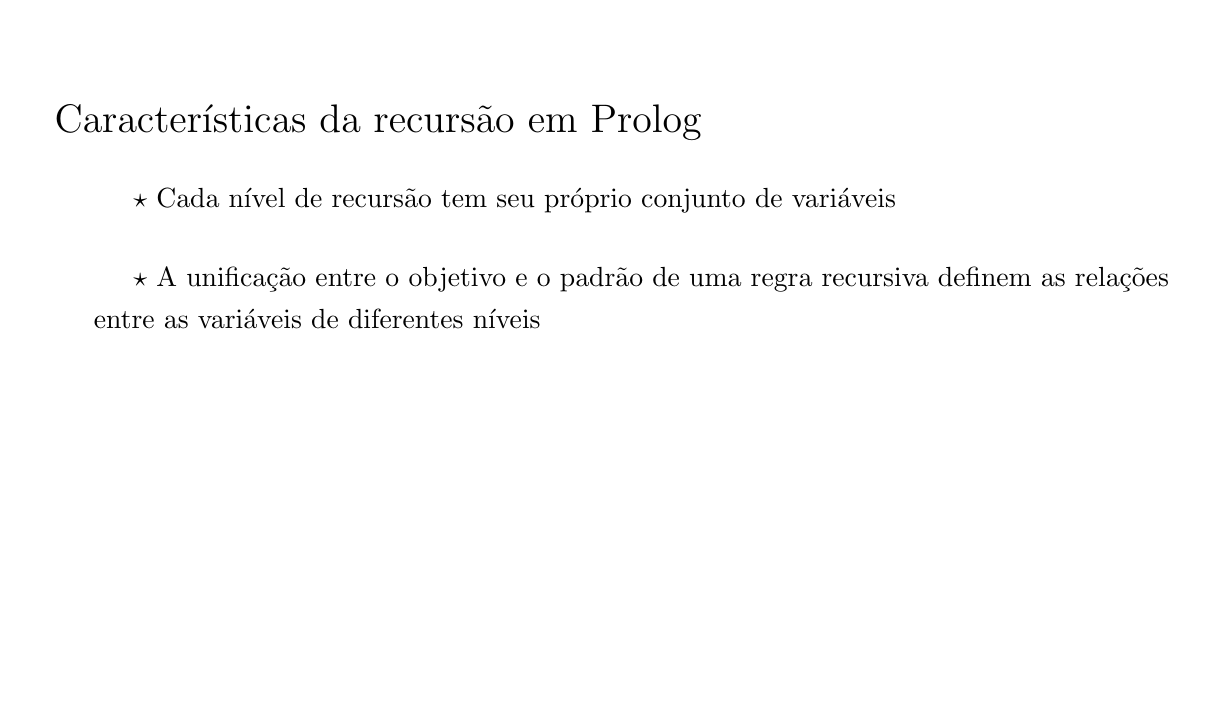
\begin{tikzpicture}
\node[draw,opacity=0] at (0, 0) {x};
\node[draw,opacity=0] at (14, 8) {x};

	\node[anchor=west] (title) at (0.0, 7.0) { \Large \bbbold{Características da recursão em Prolog} };

	\node[anchor=west] (a) at (1.0, 6.0) { $\star$ \bbtext{Cada nível de recursão tem seu próprio conjunto de variáveis} };

	\node[anchor=west] (b) at (1.0, 5.0) { $\star$ \bbtext{A unificação entre o objetivo e o padrão de uma regra recursiva definem as relações} };

	\node[anchor=west] (b1) at (0.5, 4.5) { \bbtext{entre as variáveis de diferentes níveis} };

\end{tikzpicture}
\end{frame}
\begin{frame}[plain,t]
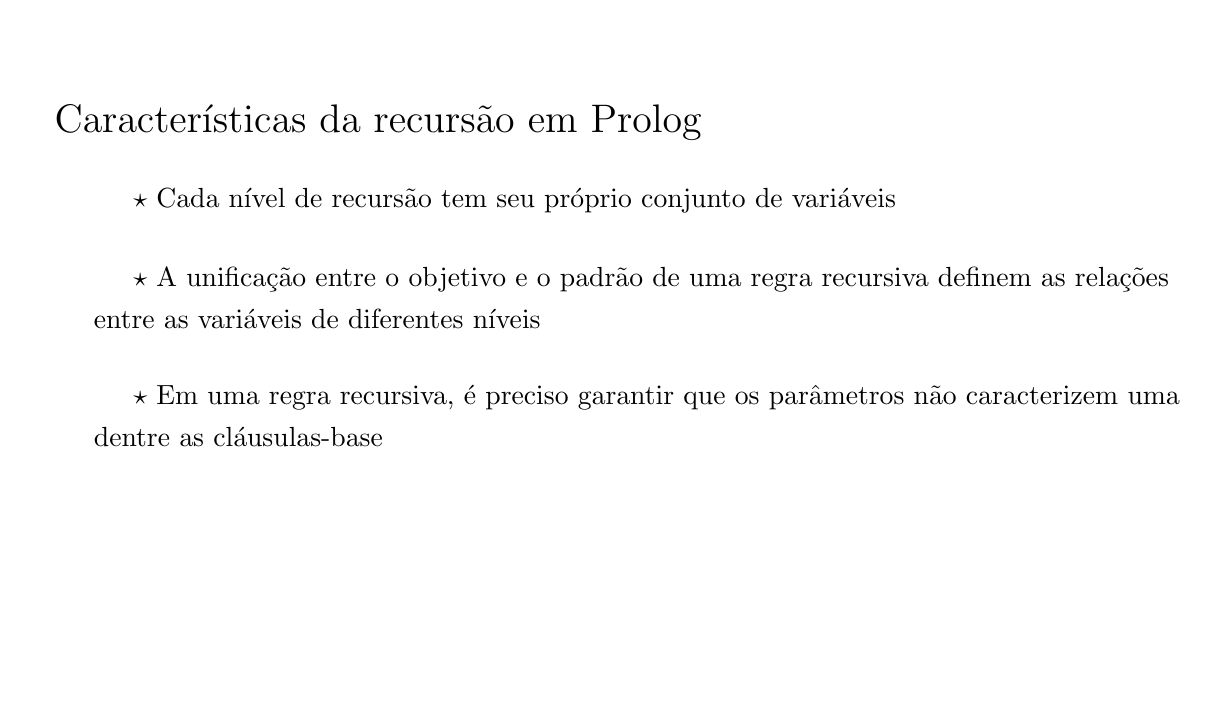
\begin{tikzpicture}
\node[draw,opacity=0] at (0, 0) {x};
\node[draw,opacity=0] at (14, 8) {x};

	\node[anchor=west] (title) at (0.0, 7.0) { \Large \bbbold{Características da recursão em Prolog} };

	\node[anchor=west] (a) at (1.0, 6.0) { $\star$ \bbtext{Cada nível de recursão tem seu próprio conjunto de variáveis} };

	\node[anchor=west] (b) at (1.0, 5.0) { $\star$ \bbtext{A unificação entre o objetivo e o padrão de uma regra recursiva definem as relações} };

	\node[anchor=west] (b1) at (0.5, 4.5) { \bbtext{entre as variáveis de diferentes níveis} };

	\node[anchor=west] (c) at (1.0, 3.5) { $\star$ \bbtext{Em uma regra recursiva, é preciso garantir que os parâmetros não caracterizem uma} };

	\node[anchor=west] (c1) at (0.5, 3.0) { \bbtext{dentre as cláusulas-base} };

\end{tikzpicture}
\end{frame}
\begin{frame}[plain,t]
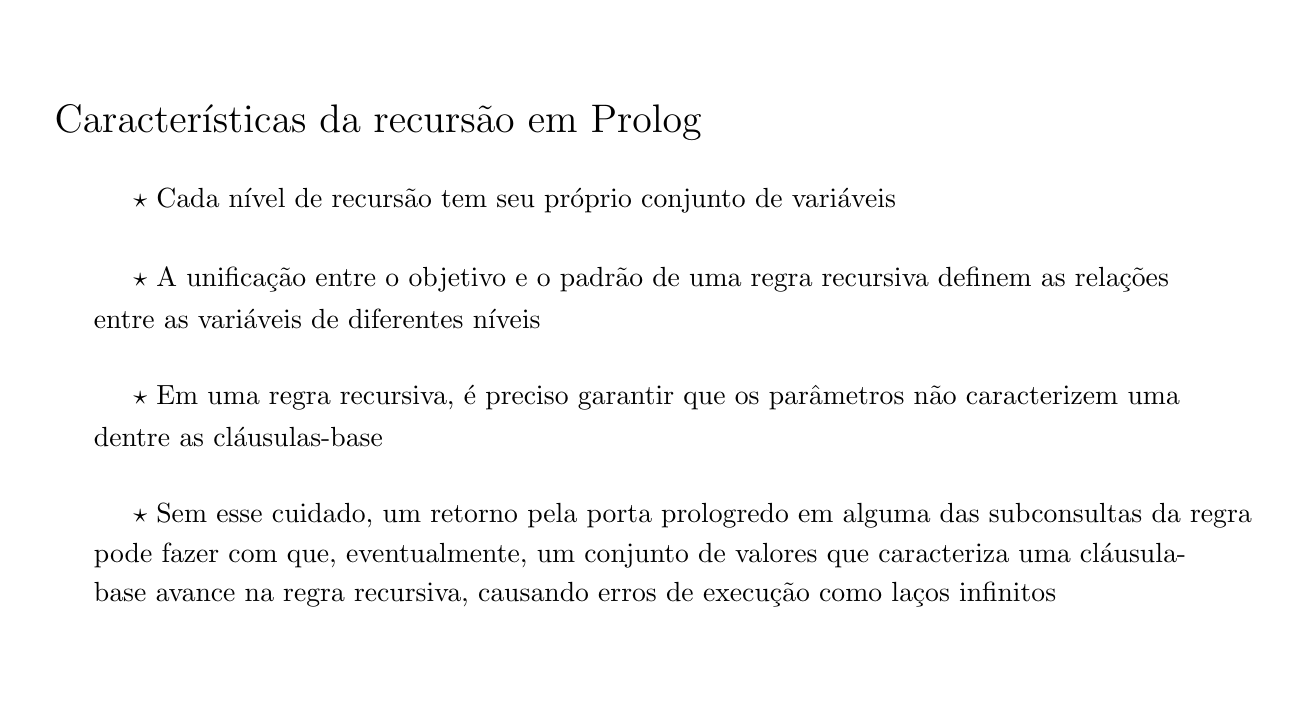
\begin{tikzpicture}
\node[draw,opacity=0] at (0, 0) {x};
\node[draw,opacity=0] at (14, 8) {x};

	\node[anchor=west] (title) at (0.0, 7.0) { \Large \bbbold{Características da recursão em Prolog} };

	\node[anchor=west] (a) at (1.0, 6.0) { $\star$ \bbtext{Cada nível de recursão tem seu próprio conjunto de variáveis} };

	\node[anchor=west] (b) at (1.0, 5.0) { $\star$ \bbtext{A unificação entre o objetivo e o padrão de uma regra recursiva definem as relações} };

	\node[anchor=west] (b1) at (0.5, 4.5) { \bbtext{entre as variáveis de diferentes níveis} };

	\node[anchor=west] (c) at (1.0, 3.5) { $\star$ \bbtext{Em uma regra recursiva, é preciso garantir que os parâmetros não caracterizem uma} };

	\node[anchor=west] (c1) at (0.5, 3.0) { \bbtext{dentre as cláusulas-base} };

	\node[anchor=west] (d) at (1.0, 2.0) { $\star$ \bbtext{Sem esse cuidado, um retorno pela porta \code{prolog}{redo} em alguma das subconsultas da regra} };

	\node[anchor=west] (d1) at (0.5, 1.5) { \bbtext{pode fazer com que, eventualmente, um conjunto de valores que caracteriza uma cláusula-} };

	\node[anchor=west] (d2) at (0.5, 1.0) { \bbtext{base avance na regra recursiva, causando erros de execução como laços infinitos} };

\end{tikzpicture}
\end{frame}
\begin{frame}[plain,t]
\vspace*{\fill}

\inputcode{prolog}{codes/fibo.pl}

\vspace*{\fill}
\end{frame}
\begin{frame}[plain,t]
\vspace*{\fill}

\inputcode{python}{codes/fibo.py}

\vspace*{\fill}
\end{frame}
\begin{frame}[plain,t]
\vspace*{\fill}

\inputcode{prolog}{codes/fibo2.pl}

\vspace*{\fill}
\end{frame}
\begin{frame}[plain,t]
\begin{tikzpicture}
\node[draw,opacity=0] at (0, 0) {x};
\node[draw,opacity=0] at (14, 8) {x};

	\node[anchor=west] (title) at (0.0, 7.0) { \Large \bbbold{Estruturas de dados em Prolog} };

\end{tikzpicture}
\end{frame}
\begin{frame}[plain,t]
\begin{tikzpicture}
\node[draw,opacity=0] at (0, 0) {x};
\node[draw,opacity=0] at (14, 8) {x};

	\node[anchor=west] (title) at (0.0, 7.0) { \Large \bbbold{Estruturas de dados em Prolog} };

	\node[anchor=west] (a) at (1.0, 6.0) { $\star$ \bbtext{Uma estrutura de dados combina termos primitivos (átomos, inteiros, etc) e} };

	\node[anchor=west] (a1) at (0.5, 5.5) { \bbtext{estruturas em tipos compostos} };

\end{tikzpicture}
\end{frame}
\begin{frame}[plain,t]
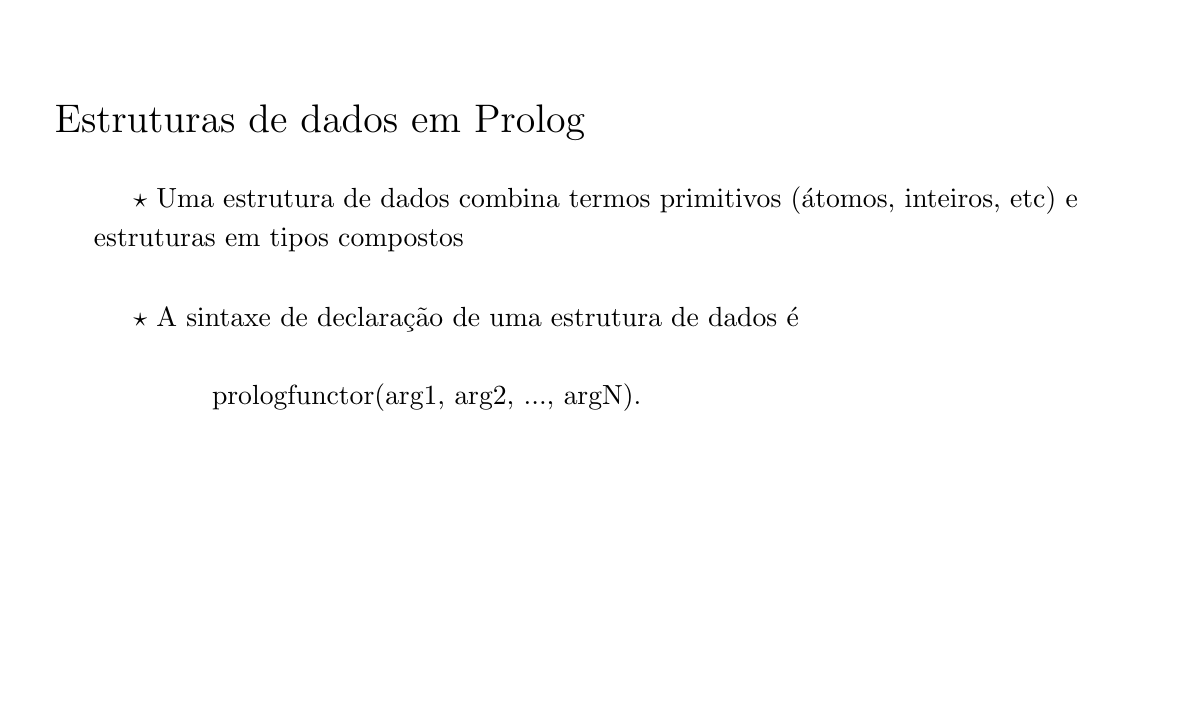
\begin{tikzpicture}
\node[draw,opacity=0] at (0, 0) {x};
\node[draw,opacity=0] at (14, 8) {x};

	\node[anchor=west] (title) at (0.0, 7.0) { \Large \bbbold{Estruturas de dados em Prolog} };

	\node[anchor=west] (a) at (1.0, 6.0) { $\star$ \bbtext{Uma estrutura de dados combina termos primitivos (átomos, inteiros, etc) e} };

	\node[anchor=west] (a1) at (0.5, 5.5) { \bbtext{estruturas em tipos compostos} };

	\node[anchor=west] (b) at (1.0, 4.5) { $\star$ \bbtext{A sintaxe de declaração de uma estrutura de dados é} };

	\node[anchor=west] (b1) at (2.0, 3.5) { \code{prolog}{functor(arg1, arg2, ..., argN).} };

\end{tikzpicture}
\end{frame}
\begin{frame}[plain,t]
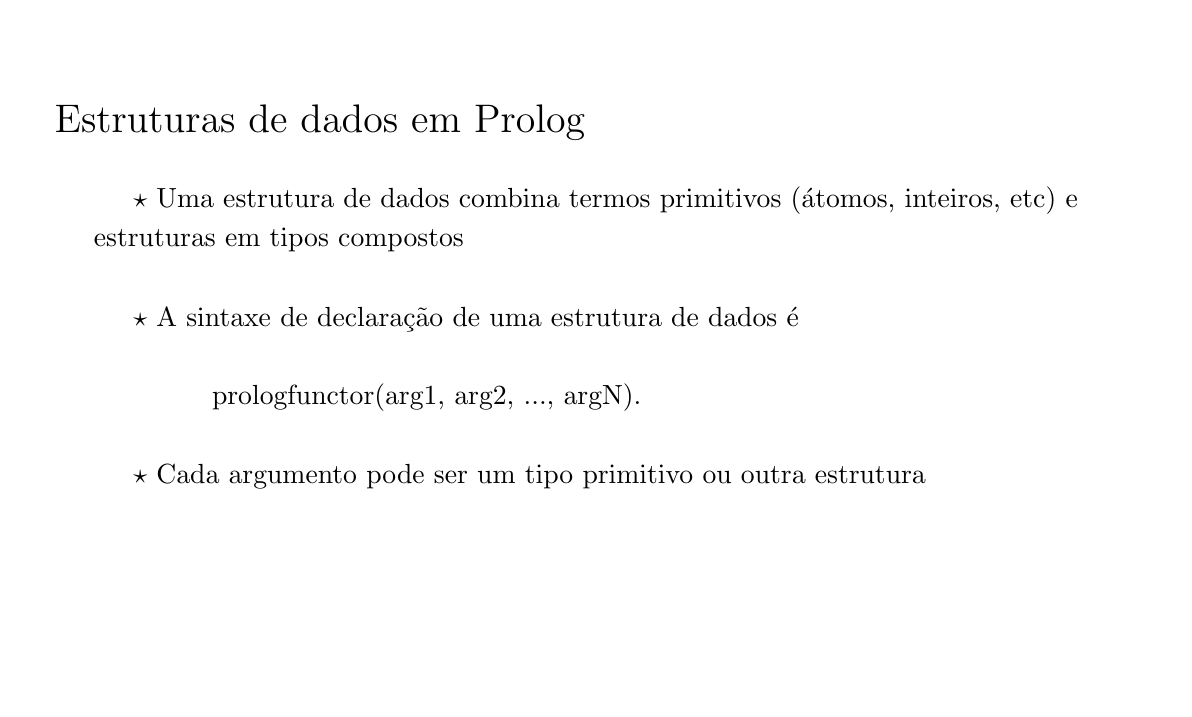
\begin{tikzpicture}
\node[draw,opacity=0] at (0, 0) {x};
\node[draw,opacity=0] at (14, 8) {x};

	\node[anchor=west] (title) at (0.0, 7.0) { \Large \bbbold{Estruturas de dados em Prolog} };

	\node[anchor=west] (a) at (1.0, 6.0) { $\star$ \bbtext{Uma estrutura de dados combina termos primitivos (átomos, inteiros, etc) e} };

	\node[anchor=west] (a1) at (0.5, 5.5) { \bbtext{estruturas em tipos compostos} };

	\node[anchor=west] (b) at (1.0, 4.5) { $\star$ \bbtext{A sintaxe de declaração de uma estrutura de dados é} };

	\node[anchor=west] (b1) at (2.0, 3.5) { \code{prolog}{functor(arg1, arg2, ..., argN).} };

	\node[anchor=west] (c) at (1.0, 2.5) { $\star$ \bbtext{Cada argumento pode ser um tipo primitivo ou outra estrutura} };

\end{tikzpicture}
\end{frame}
\begin{frame}[plain,t]
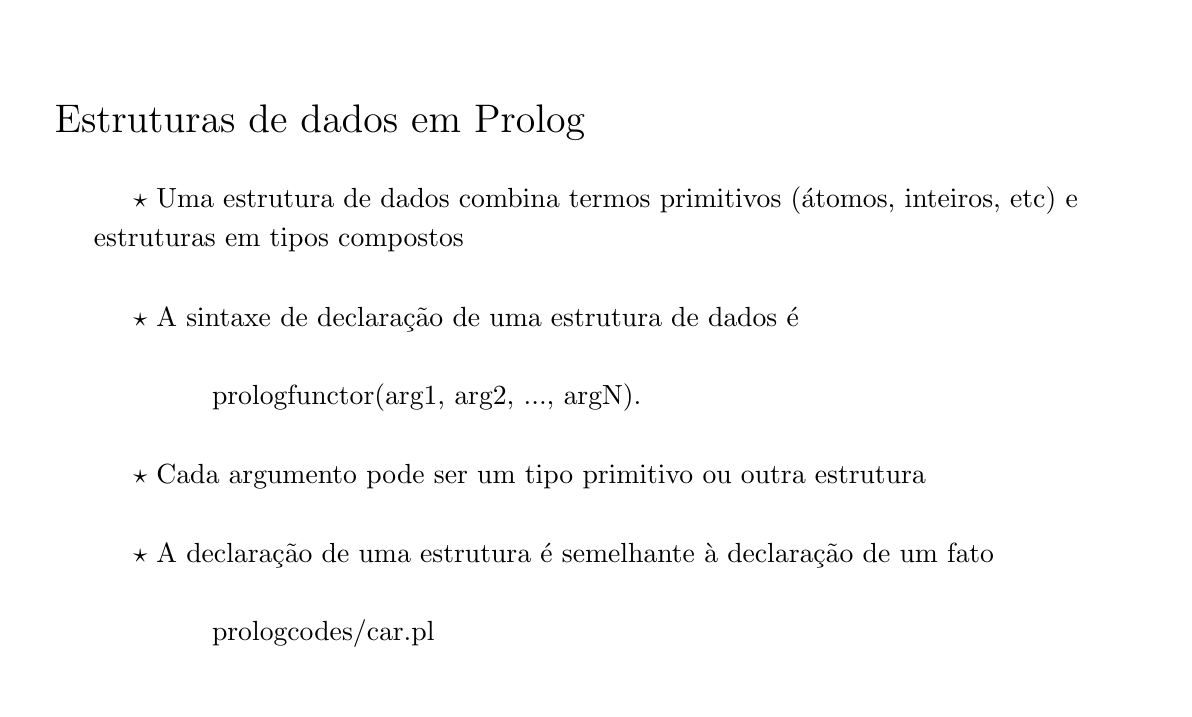
\begin{tikzpicture}
\node[draw,opacity=0] at (0, 0) {x};
\node[draw,opacity=0] at (14, 8) {x};

	\node[anchor=west] (title) at (0.0, 7.0) { \Large \bbbold{Estruturas de dados em Prolog} };

	\node[anchor=west] (a) at (1.0, 6.0) { $\star$ \bbtext{Uma estrutura de dados combina termos primitivos (átomos, inteiros, etc) e} };

	\node[anchor=west] (a1) at (0.5, 5.5) { \bbtext{estruturas em tipos compostos} };

	\node[anchor=west] (b) at (1.0, 4.5) { $\star$ \bbtext{A sintaxe de declaração de uma estrutura de dados é} };

	\node[anchor=west] (b1) at (2.0, 3.5) { \code{prolog}{functor(arg1, arg2, ..., argN).} };

	\node[anchor=west] (c) at (1.0, 2.5) { $\star$ \bbtext{Cada argumento pode ser um tipo primitivo ou outra estrutura} };

	\node[anchor=west] (d) at (1.0, 1.5) { $\star$ \bbtext{A declaração de uma estrutura é semelhante à declaração de um fato} };


	\node[anchor=west] (d1) at (2.0, 0.5) { \inputsyntax{prolog}{codes/car.pl} };

\end{tikzpicture}
\end{frame}
\begin{frame}[plain,t]
\begin{tikzpicture}
\node[draw,opacity=0] at (0, 0) {x};
\node[draw,opacity=0] at (14, 8) {x};

	\node[anchor=west] (title) at (0.0, 7.0) { \Large \bbbold{Consultas envolvendo estruturas de dados} };

\end{tikzpicture}
\end{frame}
\begin{frame}[plain,t]
\begin{tikzpicture}
\node[draw,opacity=0] at (0, 0) {x};
\node[draw,opacity=0] at (14, 8) {x};

	\node[anchor=west] (title) at (0.0, 7.0) { \Large \bbbold{Consultas envolvendo estruturas de dados} };

	\node[anchor=west] (a) at (1.0, 6.0) { $\star$ \bbtext{A ordem dos argumentos influencia o resultado de um consulta} };

	\node[anchor=west] (a1) at (2.0, 5.0) { \code{prolog}{car(X, red, _).} };

\end{tikzpicture}
\end{frame}
\begin{frame}[plain,t]
\begin{tikzpicture}
\node[draw,opacity=0] at (0, 0) {x};
\node[draw,opacity=0] at (14, 8) {x};

	\node[anchor=west] (title) at (0.0, 7.0) { \Large \bbbold{Consultas envolvendo estruturas de dados} };

	\node[anchor=west] (a) at (1.0, 6.0) { $\star$ \bbtext{A ordem dos argumentos influencia o resultado de um consulta} };

	\node[anchor=west] (a1) at (2.0, 5.0) { \code{prolog}{car(X, red, _).} };

	\node[anchor=west] (b) at (1.0, 4.0) { $\star$ \bbtext{Campos podem ser ignorados com a variável anônima `\code{prolog}{_}'} };

\end{tikzpicture}
\end{frame}
\begin{frame}[plain,t]
\begin{tikzpicture}
\node[draw,opacity=0] at (0, 0) {x};
\node[draw,opacity=0] at (14, 8) {x};

	\node[anchor=west] (title) at (0.0, 7.0) { \Large \bbbold{Consultas envolvendo estruturas de dados} };

	\node[anchor=west] (a) at (1.0, 6.0) { $\star$ \bbtext{A ordem dos argumentos influencia o resultado de um consulta} };

	\node[anchor=west] (a1) at (2.0, 5.0) { \code{prolog}{car(X, red, _).} };

	\node[anchor=west] (b) at (1.0, 4.0) { $\star$ \bbtext{Campos podem ser ignorados com a variável anônima `\code{prolog}{_}'} };

	\node[anchor=west] (c) at (1.0, 3.0) { $\star$ \bbtext{Estruturas podem ser aninhadas, com o intuito de aumentar a legibilidade} };

	\node[anchor=west] (c1) at (2.0, 2.0) { \code{prolog}{car(honda, color(red), doors(4)).} };

\end{tikzpicture}
\end{frame}
\begin{frame}[plain,t]
\begin{tikzpicture}
\node[draw,opacity=0] at (0, 0) {x};
\node[draw,opacity=0] at (14, 8) {x};

	\node[anchor=west] (title) at (0.0, 7.0) { \Large \bbbold{Consultas envolvendo estruturas de dados} };

	\node[anchor=west] (a) at (1.0, 6.0) { $\star$ \bbtext{A ordem dos argumentos influencia o resultado de um consulta} };

	\node[anchor=west] (a1) at (2.0, 5.0) { \code{prolog}{car(X, red, _).} };

	\node[anchor=west] (b) at (1.0, 4.0) { $\star$ \bbtext{Campos podem ser ignorados com a variável anônima `\code{prolog}{_}'} };

	\node[anchor=west] (c) at (1.0, 3.0) { $\star$ \bbtext{Estruturas podem ser aninhadas, com o intuito de aumentar a legibilidade} };

	\node[anchor=west] (c1) at (2.0, 2.0) { \code{prolog}{car(honda, color(red), doors(4)).} };

	\node[anchor=west] (d) at (1.0, 1.0) { $\star$ \bbtext{As duas cláusulas acima não unificam} };

\end{tikzpicture}
\end{frame}
\begin{frame}[plain,t]
\vspace*{\fill}

\inputsnippet{prolog}{1}{17}{codes/matrioskas.pl}

\vspace*{\fill}
\end{frame}
\begin{frame}[plain,t]
\vspace*{\fill}

\inputsnippet{prolog}{19}{32}{codes/matrioskas.pl}

\vspace*{\fill}
\end{frame}
\begin{frame}[plain,t]
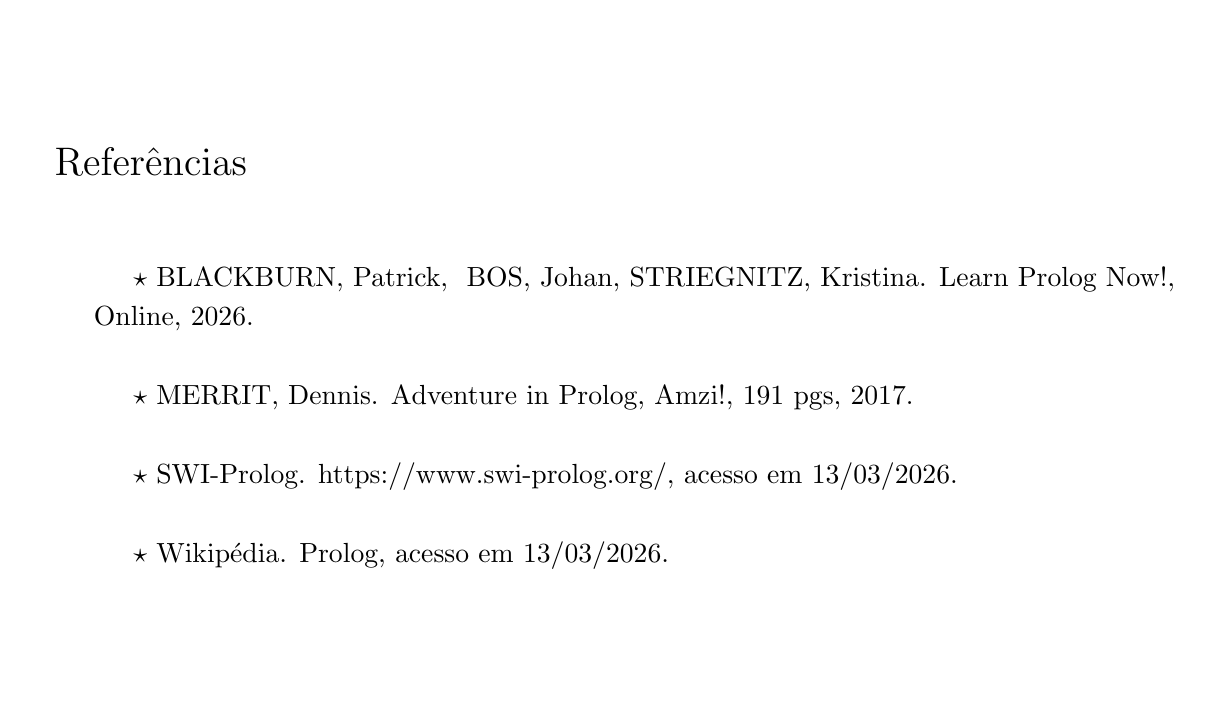
\begin{tikzpicture}
\node[draw,opacity=0] at (0, 0) {x};
\node[draw,opacity=0] at (14, 8) {x};

	\node[anchor=west] (title) at (0.0, 6.5) { \Large \bbbold{Referências} };

	\node[anchor=west] (a) at (1.0, 2.5) { $\star$ \bbbold{SWI-Prolog.} \bbenglish{https://www.swi-prolog.org/,} \bbtext{acesso em 13/03/2026.} };

	\node[anchor=west] (c) at (1.0, 1.5) { $\star$ \bbbold{Wikipédia.} \bbenglish{Prolog,} \bbtext{acesso em 13/03/2026.} };

	\node[anchor=west] (d) at (1.0, 3.5) { $\star$ \bbbold{MERRIT}\bbtext{, Dennis.} \bbenglish{Adventure in Prolog, Amzi!,} \bbtext{191 pgs, 2017.} };

	\node[anchor=west] (e) at (1.0, 5.0) { $\star$ \bbbold{BLACKBURN}\bbtext{, Patrick, } \bbbold{BOS}\bbtext{, Johan,} \bbbold{STRIEGNITZ}, \bbtext{Kristina.} \bbenglish{Learn Prolog Now!,} };

	\node[anchor=west] (e1) at (0.5, 4.5) { \bbtext{Online, 2026.} };


\end{tikzpicture}
\end{frame}
\end{document}
